\documentclass[11pt]{article}
\usepackage{array, url, kantlipsum, listings, xcolor}
\usepackage[margin=1in]{geometry}
\usepackage{graphicx, float, courier}
\usepackage[section]{placeins}
\usepackage[utf8]{inputenc}
\graphicspath{ {output/} }

\lstdefinestyle{terminal}
{
    backgroundcolor=\color{white},
    basicstyle=\footnotesize\color{black}\ttfamily,
    frame=tb,
}
\makeatletter
\long\def\@makecaption#1#2{%
	\vskip\abovecaptionskip
		\bfseries #1: #2\par
	\vskip\belowcaptionskip}%
\makeatother

\title{Assignment 3 \\CPSC 526 Fall 2017 \\ October 29, 2017}
\author{
\begin{tabular}{c c}
Mason Lieu & Shane Sims\tabularnewline
ID: 10110089 & ID: 00300601\tabularnewline
Tutorial 04 & Tutorial 04 \tabularnewline
\url{mlieu@ucalgary.ca} & \url{shane.sims@ucalgary.ca}
\end{tabular}}
\date{}

\begin{document}
\maketitle
\tableofcontents

\section{How to monitor HTTP}
\begin{lstlisting}[style=terminal, title={Terminal 1: Run the proxy server}]
python3 simpleProxyServer.py [log options] <source port> <web server URL> <destination port>
\end{lstlisting}
\begin{lstlisting}[style=terminal, title={Web browser: Connect to the server}]
localhost:<source port>
\end{lstlisting}

\section{How to monitor SSH}
\begin{lstlisting}[style=terminal, title={Terminal 1: Run the proxy server}]
python3 simpleProxyServer.py [log options] <source port> localhost 22
\end{lstlisting}
\begin{lstlisting}[style=terminal, title={Terminal 2: Connect to the server through SSH}]
ssh localhost -p 22
\end{lstlisting}

\section{How to monitor NetCat-to-NetCat}
\begin{lstlisting}[style=terminal, title={Terminal 1: Run NetCat to listen for incoming connections}]
nc -l <destination port>
\end{lstlisting}
\begin{lstlisting}[style=terminal, title={Terminal 2: Run the proxy server}]
python3 simpleProxyServer.py [log options] <source port> localhost <destination port>
\end{lstlisting}
\begin{lstlisting}[style=terminal, title={Terminal 3: Run NetCat}]
nc localhost <source port>
\end{lstlisting}

\section{Supported logging formats}
This program supports the following logging formats
\begin{enumerate}
\item -raw
\item -strip
\item -hex
\item -autoN
\item -replace
\end{enumerate}

\section{Sample output}

	\subsection{Output - no logging}
	\begin{figure}[H]
	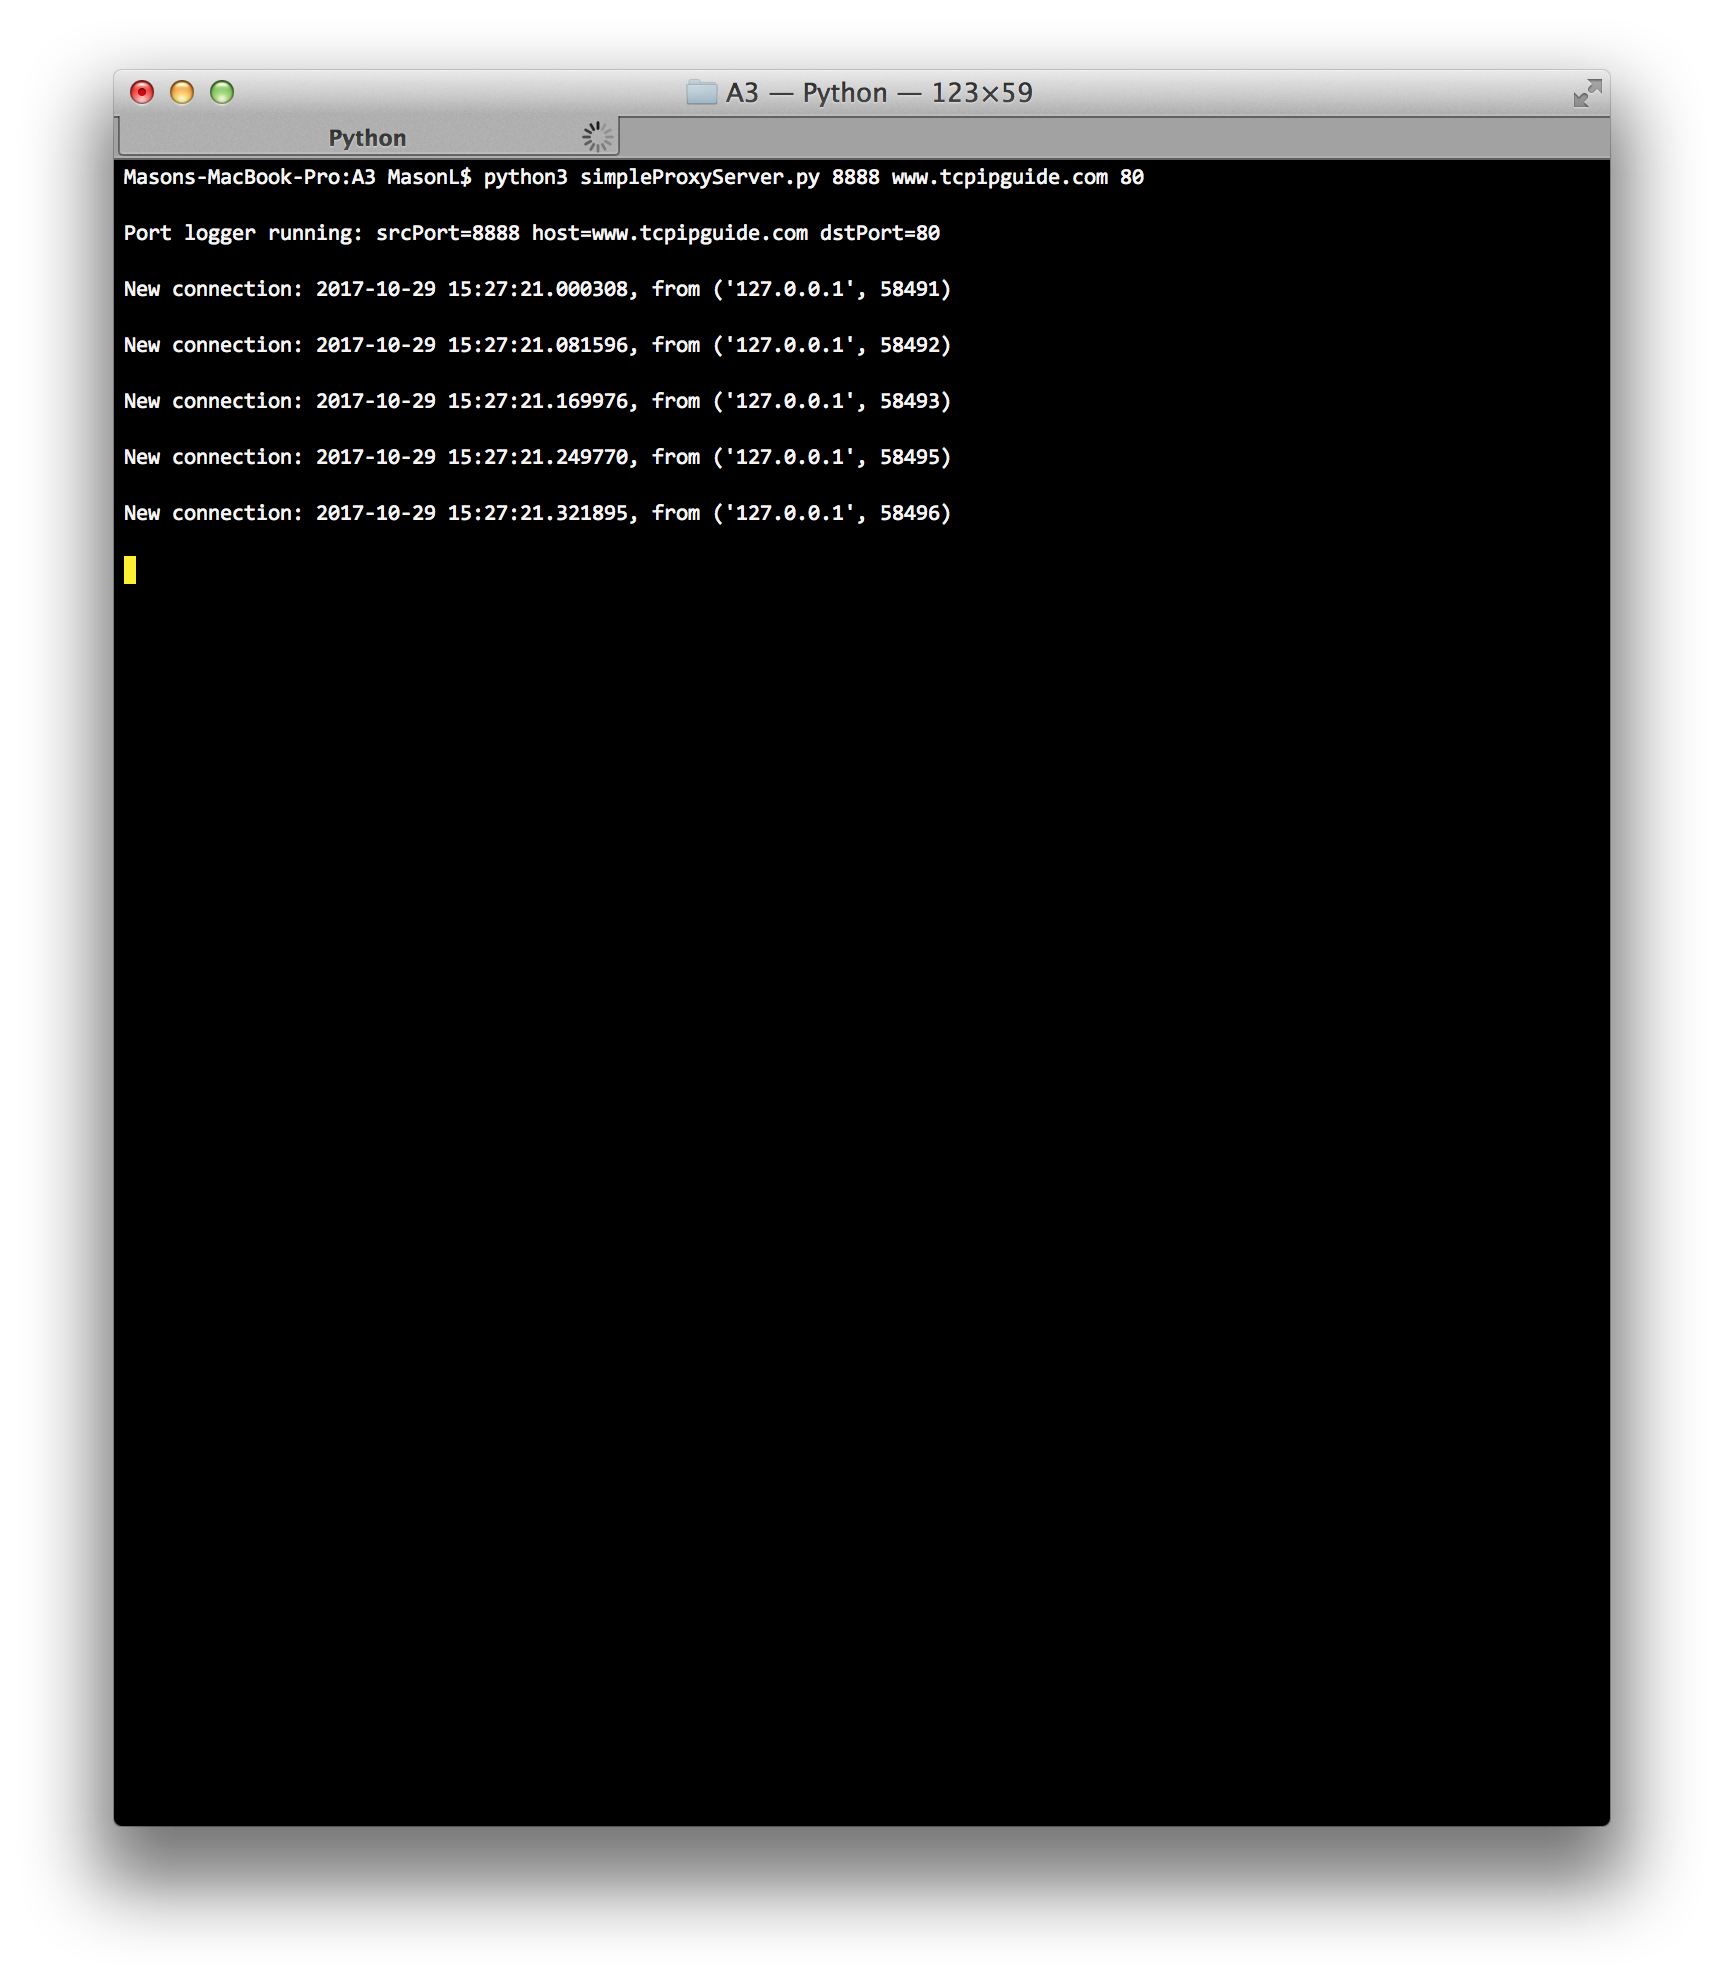
\includegraphics[scale=0.5, trim={0cm 0cm 0cm 0cm}, clip]{none_output}
	\caption{No logging options selected}
	\end{figure}
	
	\subsection{Output - raw}
	\begin{figure}[H]
	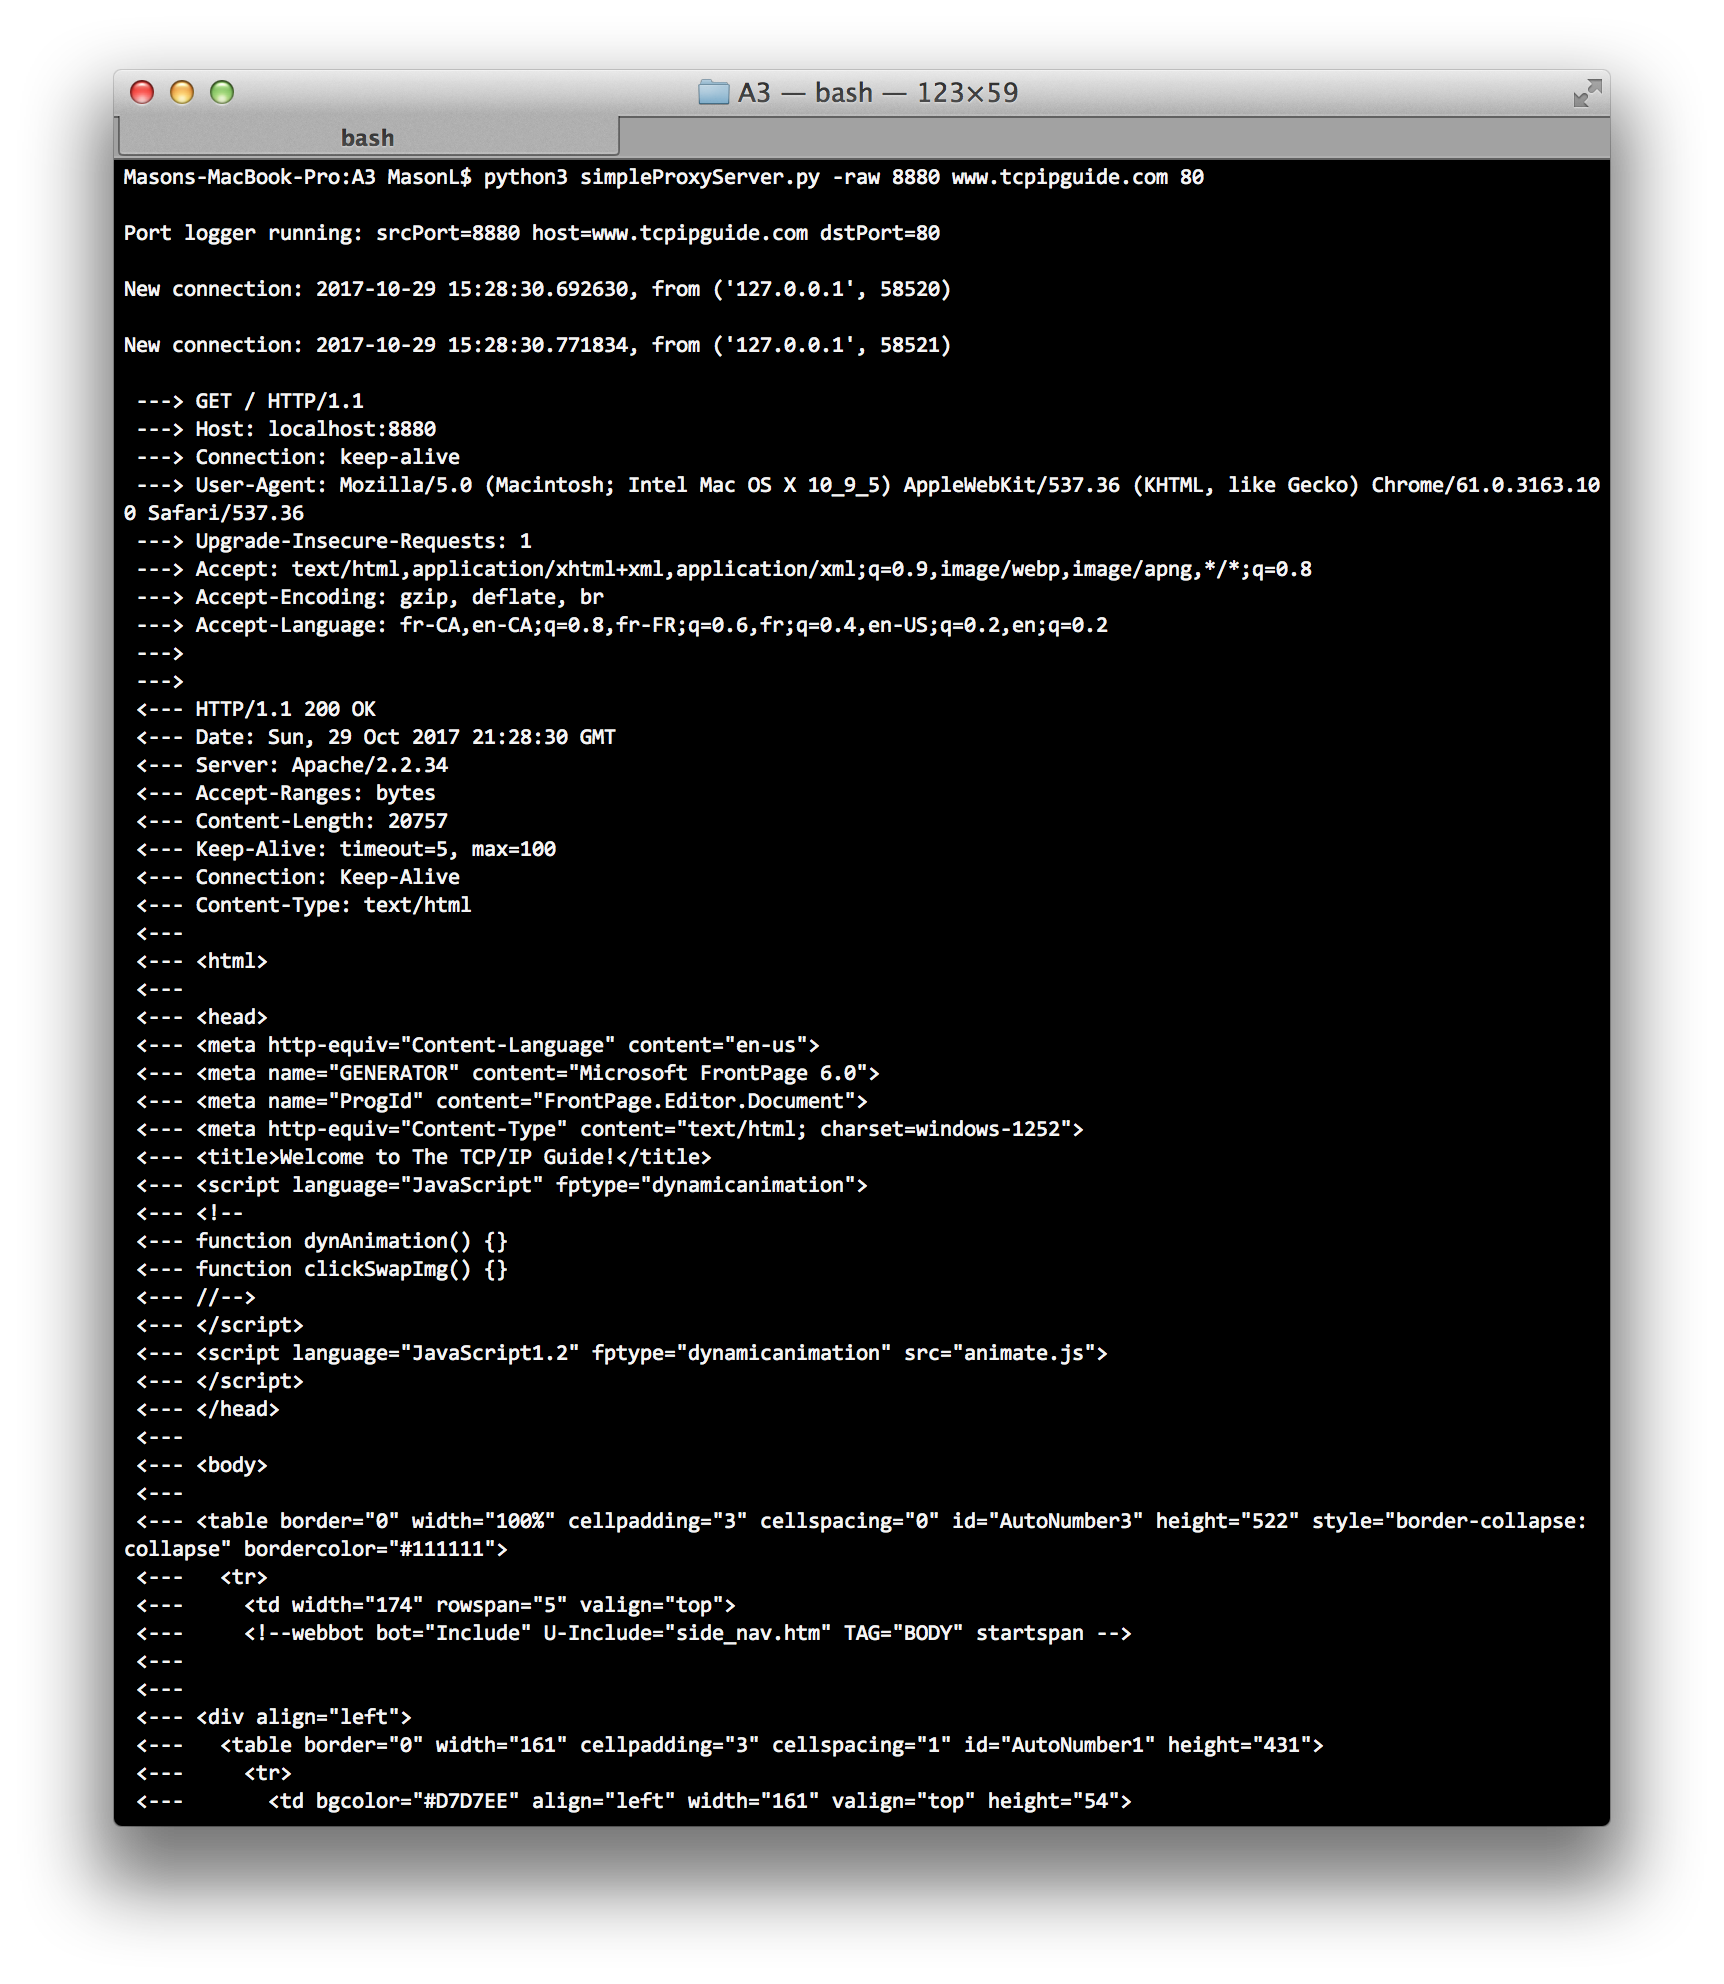
\includegraphics[scale=0.5, trim={0cm 0cm 0cm 0cm}, clip]{raw_output}
	\caption{Initialization of proxy server with raw formatting}
	\end{figure}
	\begin{figure}[H]
	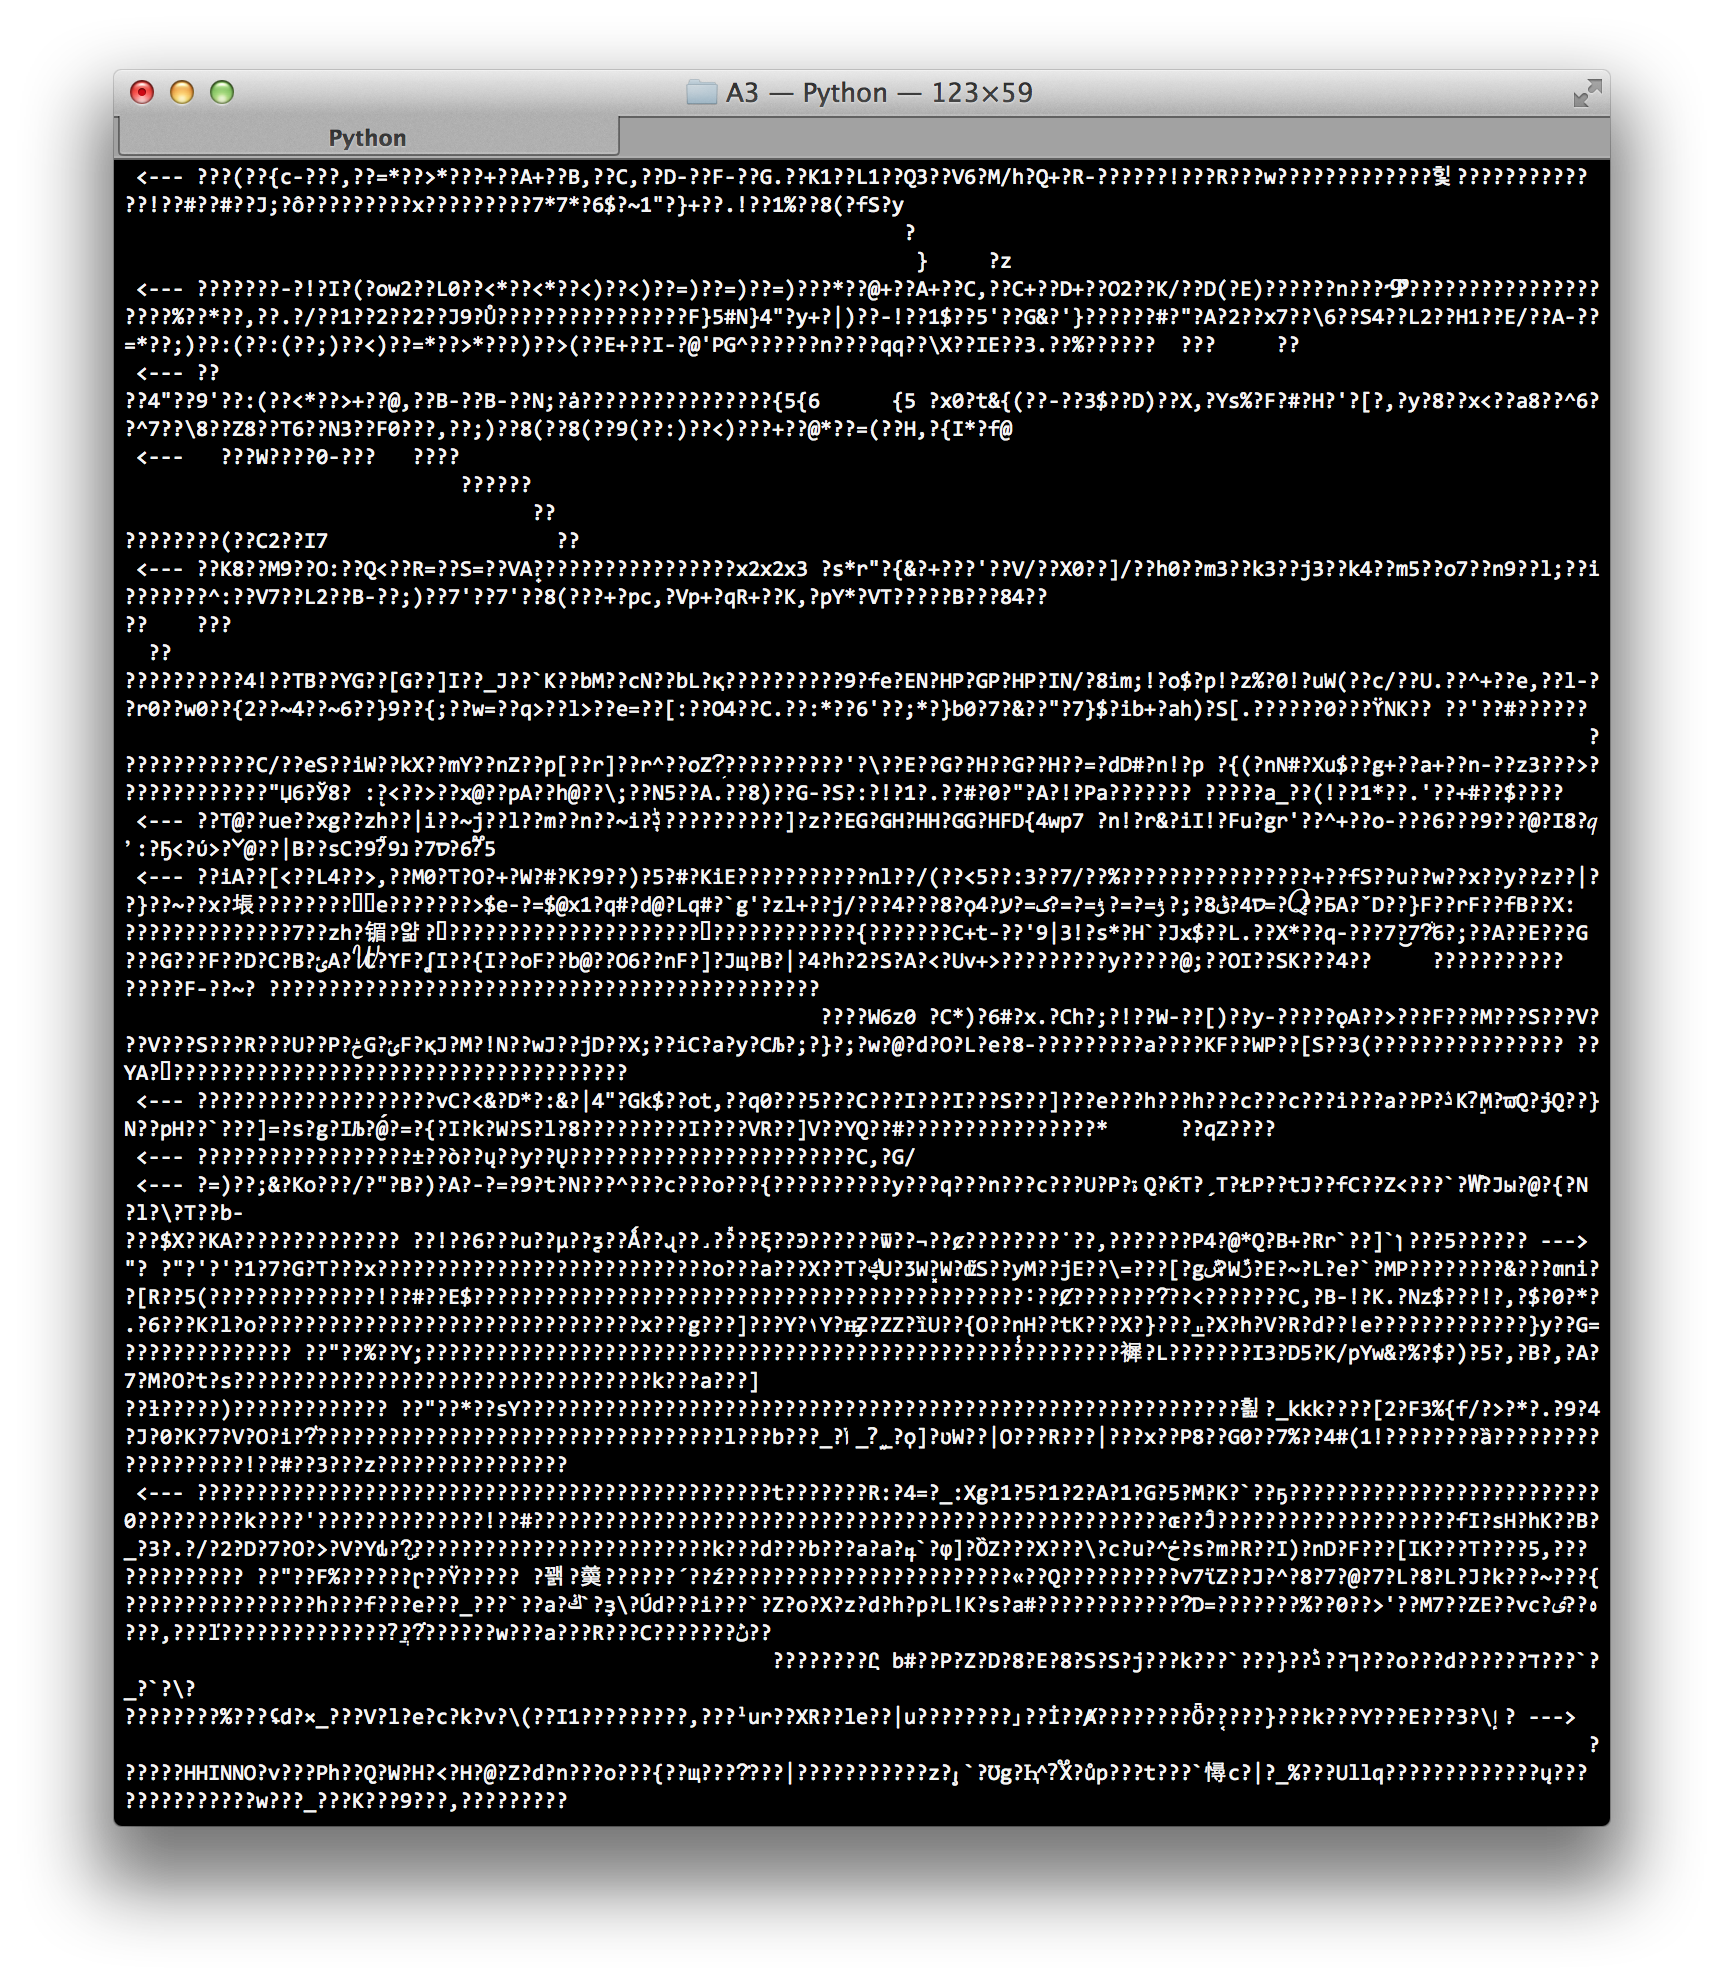
\includegraphics[scale=0.5, trim={0cm 0cm 0cm 0cm}, clip]{raw_output_mid}
	\caption{Sample output in the middle of execution}
	\end{figure}
	
	\subsection{Output - strip}
	\begin{figure}[H]
	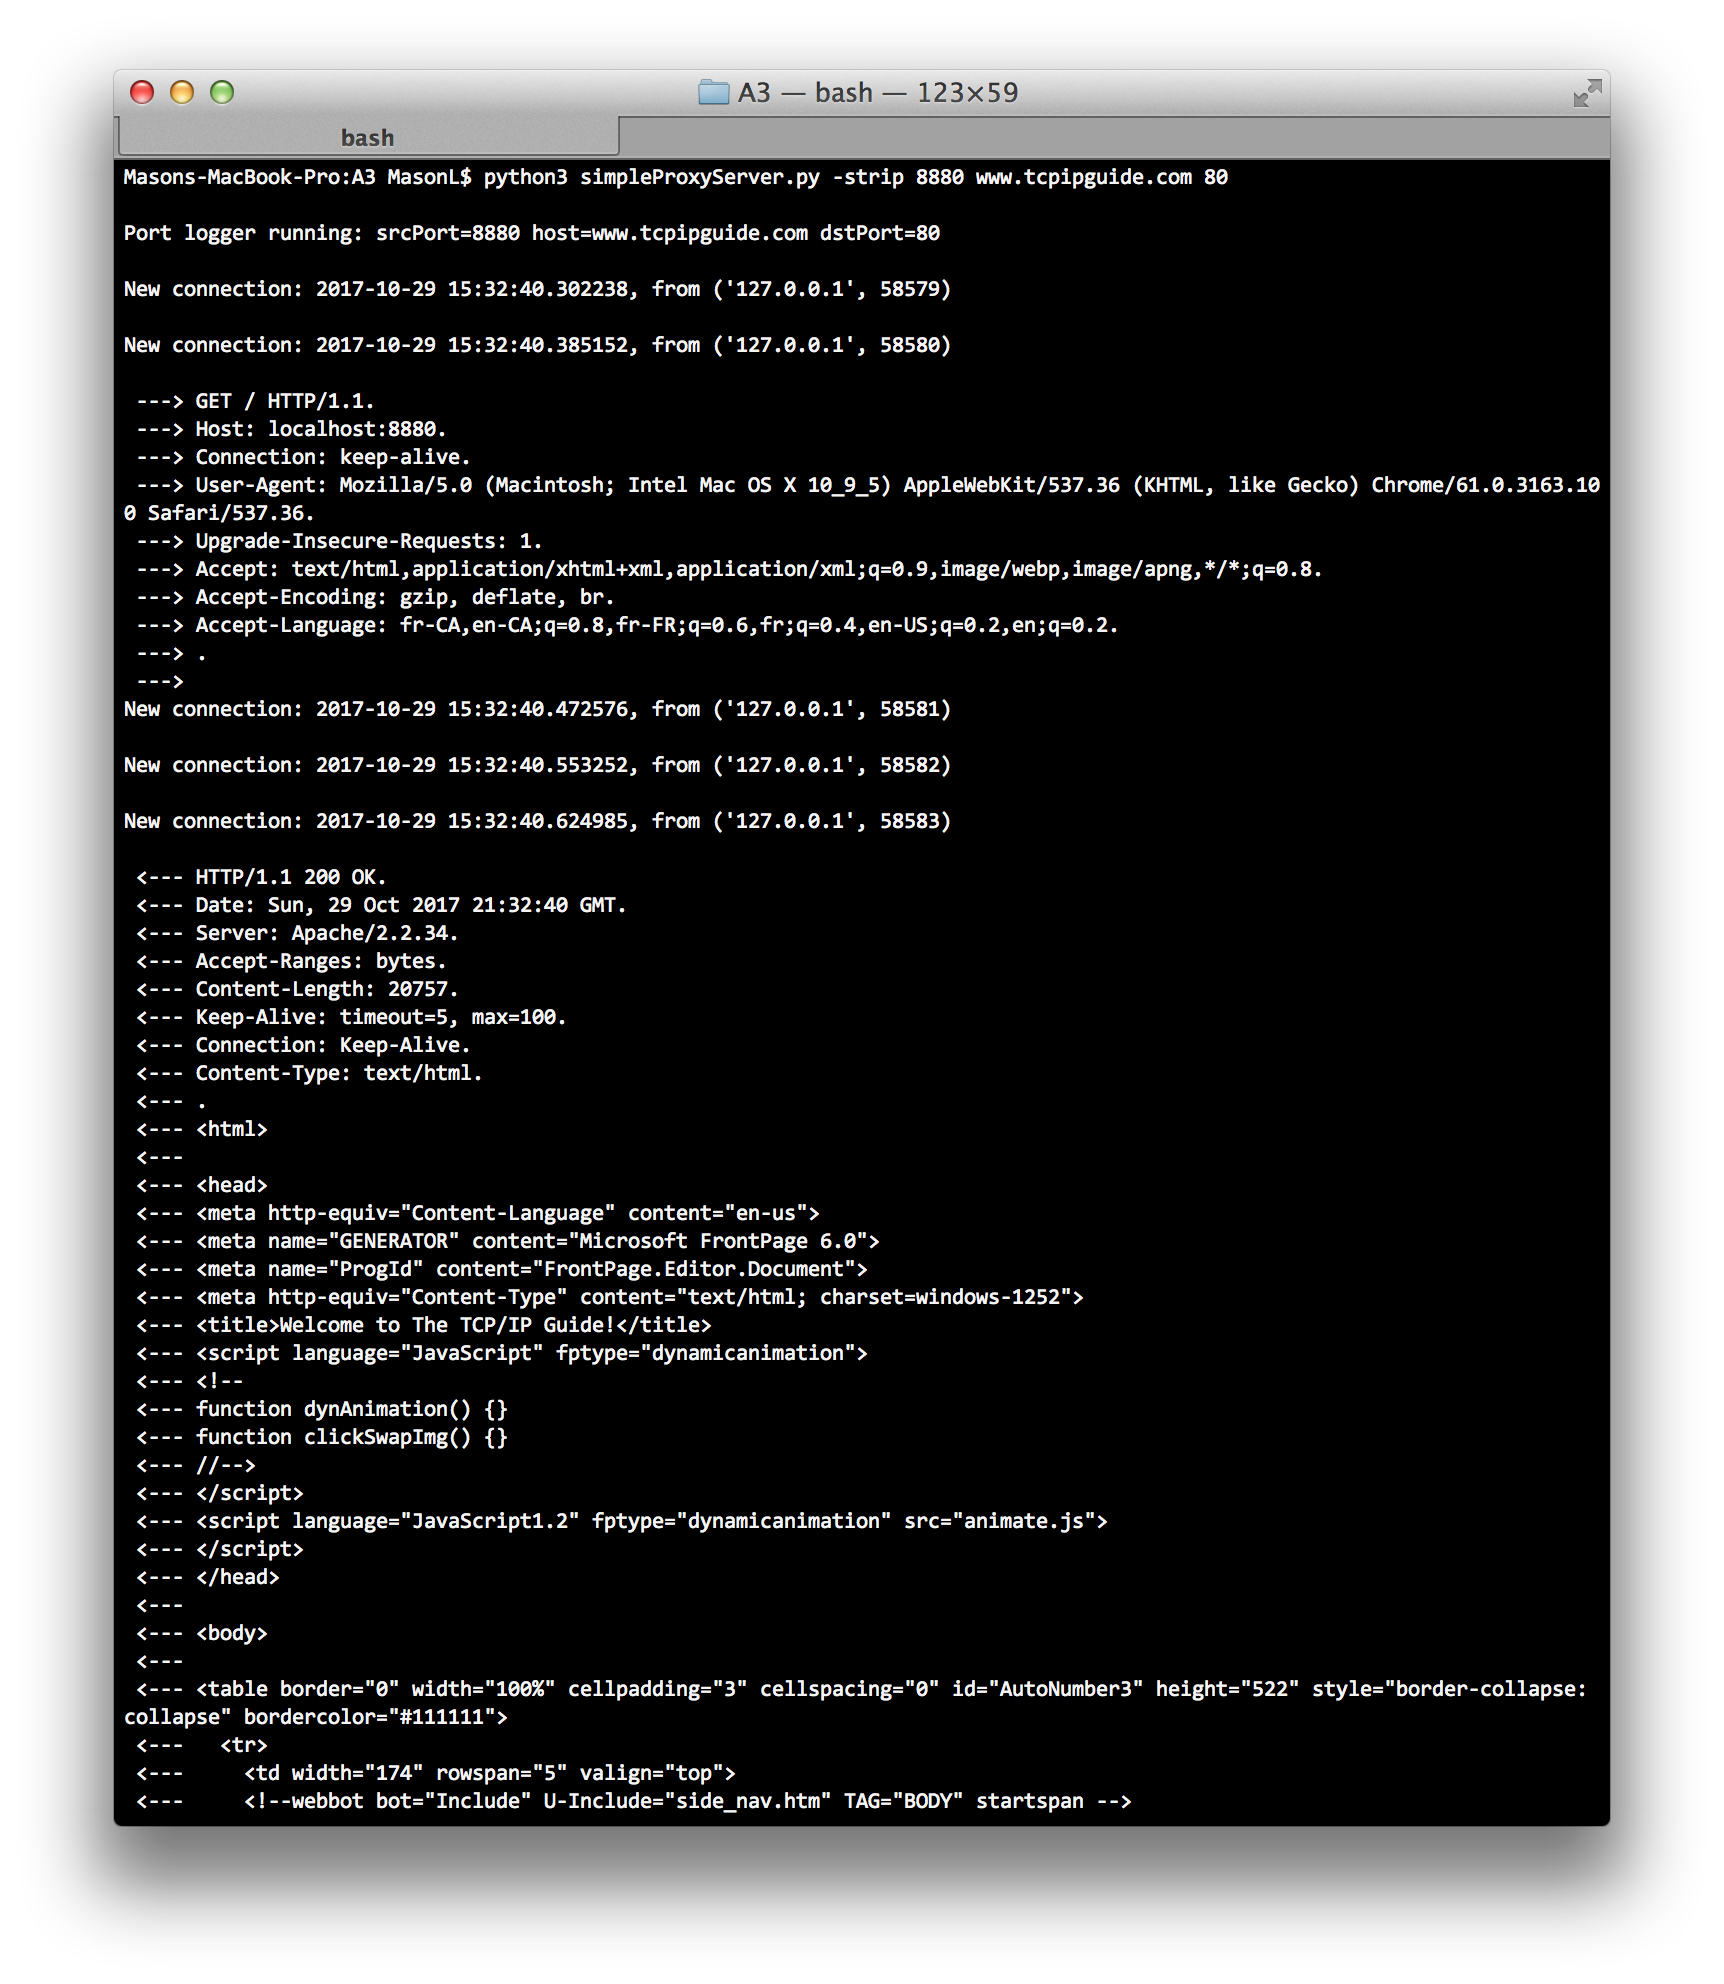
\includegraphics[scale=0.5, trim={0cm 0cm 0cm 0cm}, clip]{strip_output}
	\caption{Initialization of proxy server with strip formatting}
	\end{figure}
	\begin{figure}[H]
	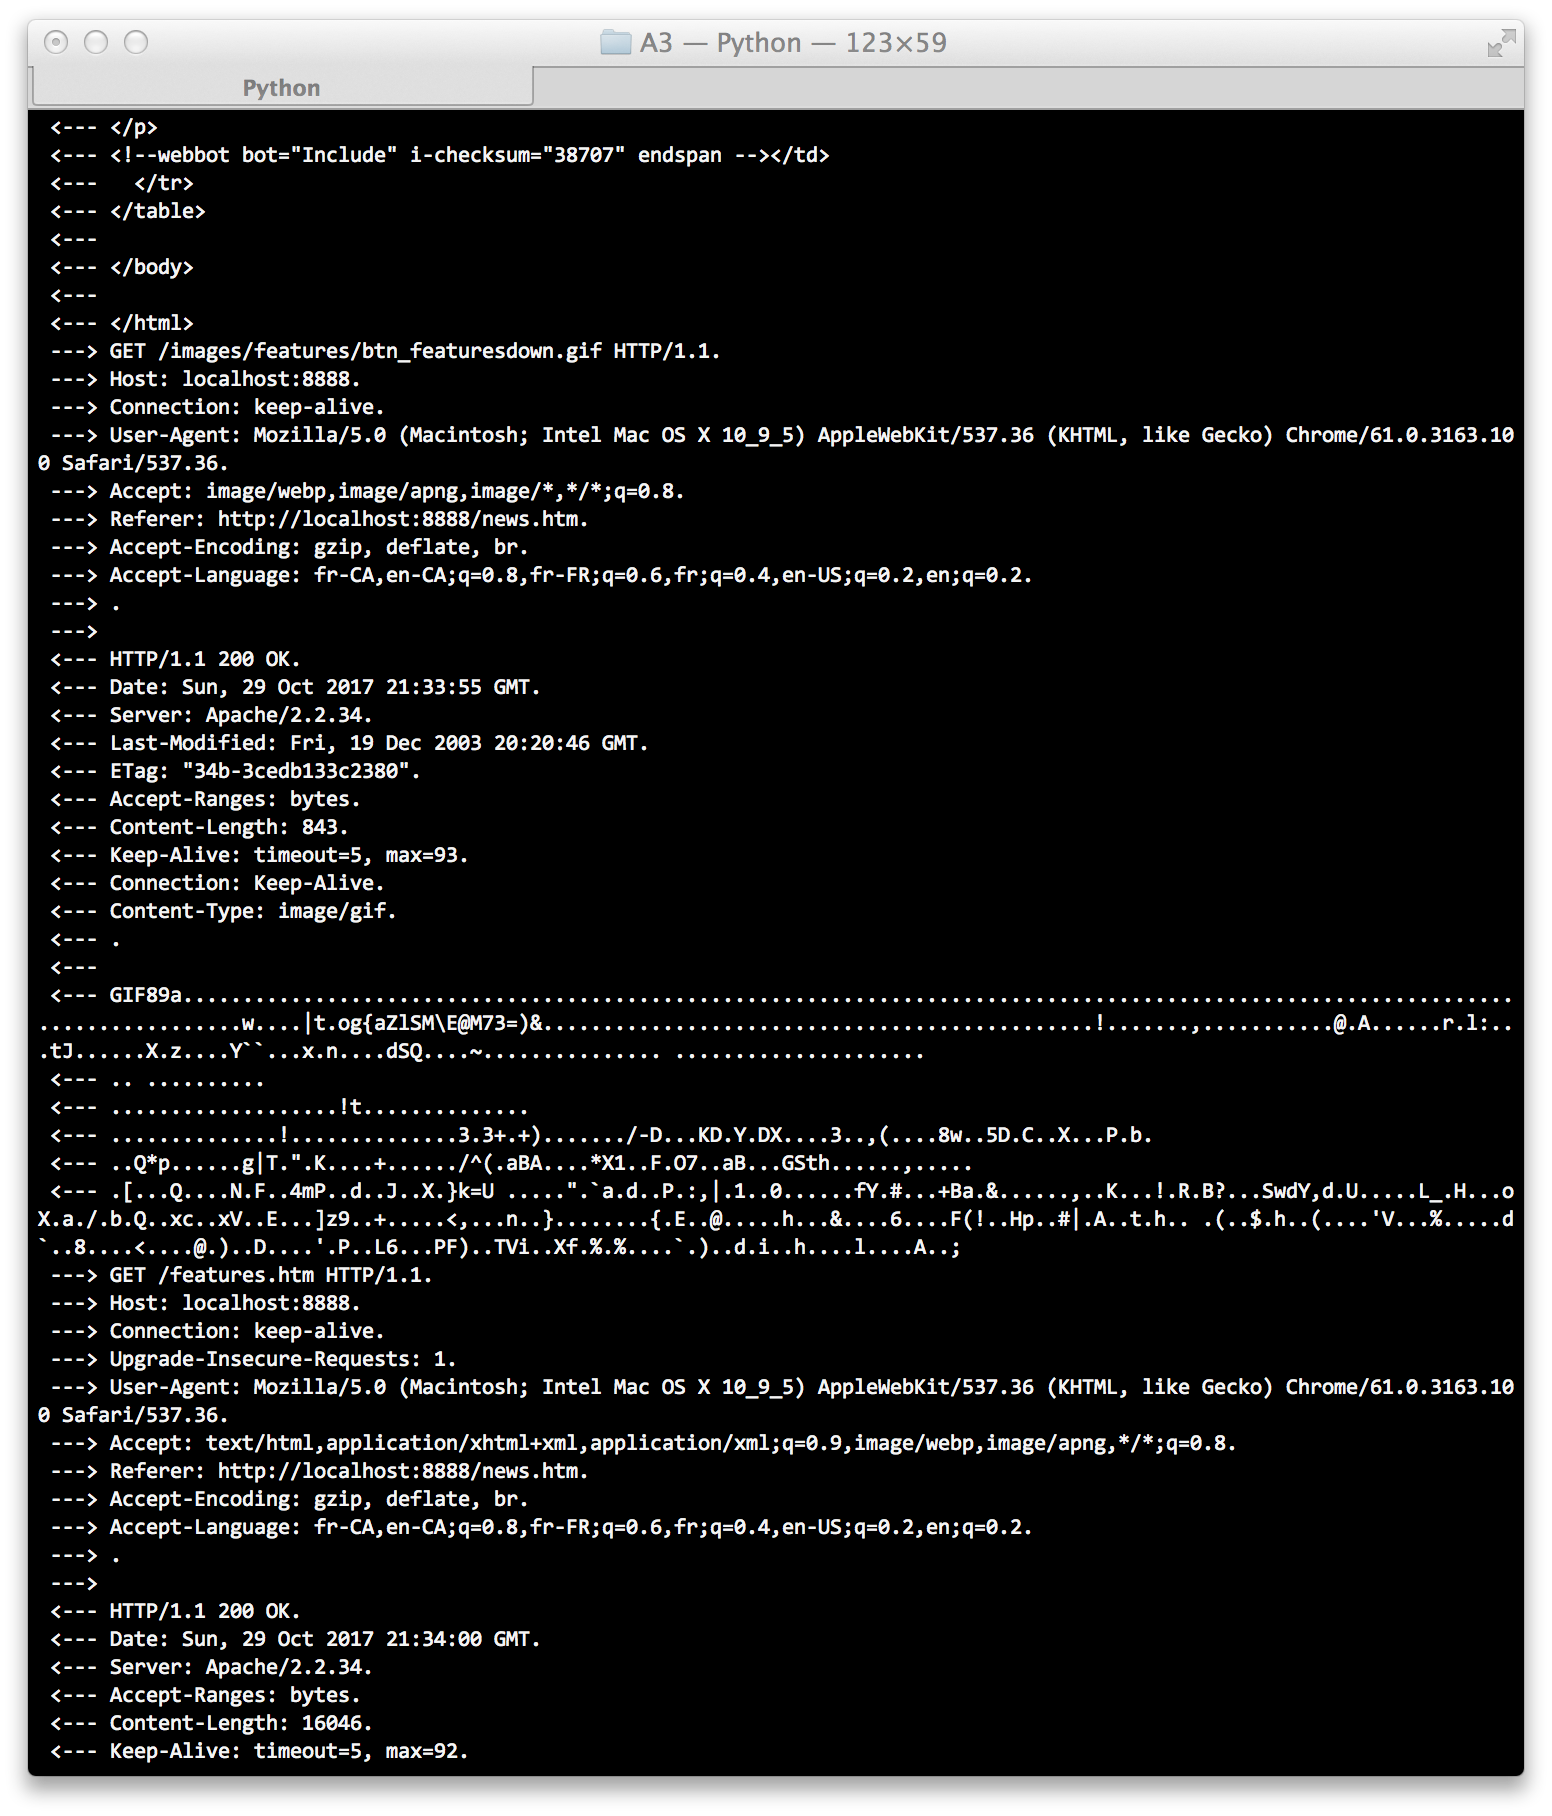
\includegraphics[scale=0.5, trim={0cm 0cm 0cm 0cm}, clip]{strip_output_mid}
	\caption{Sample output in the middle of execution}
	\end{figure}
	
	\subsection{Output - hex}
	\begin{figure}[H]
	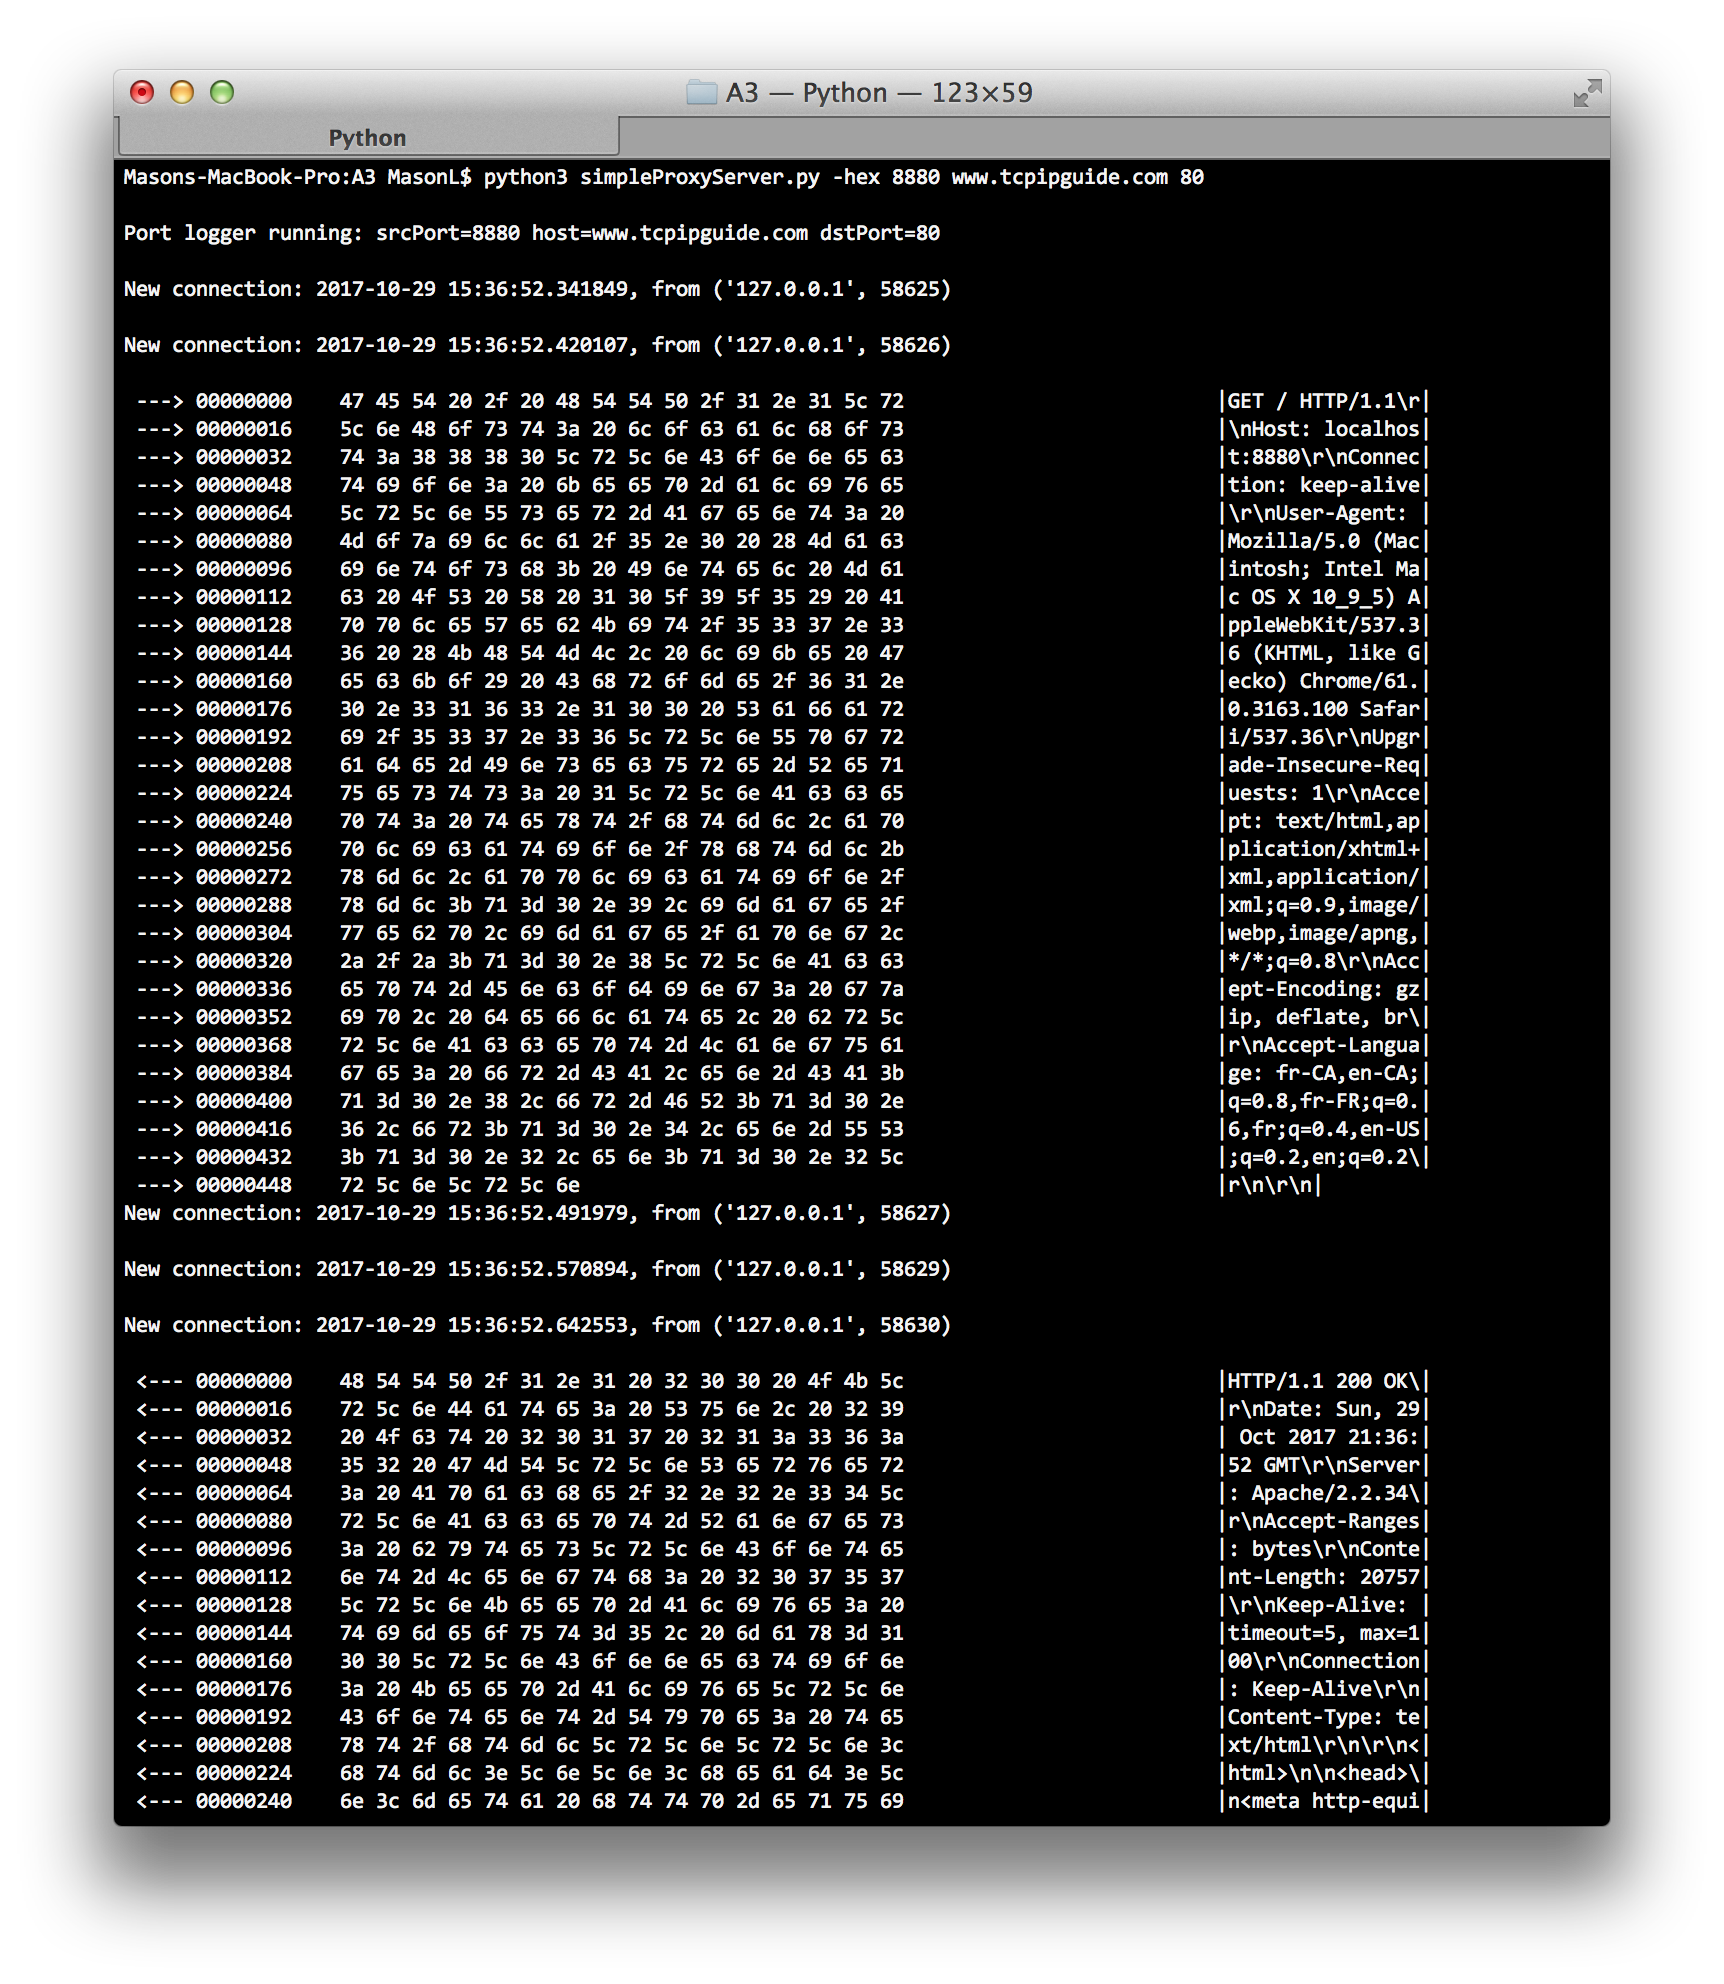
\includegraphics[scale=0.5, trim={0cm 0cm 0cm 0cm}, clip]{hex_output}
	\caption{Initialization of proxy server with hex formatting}
	\end{figure}
	
	\subsection{Output - autoN}
	\begin{figure}[H]
	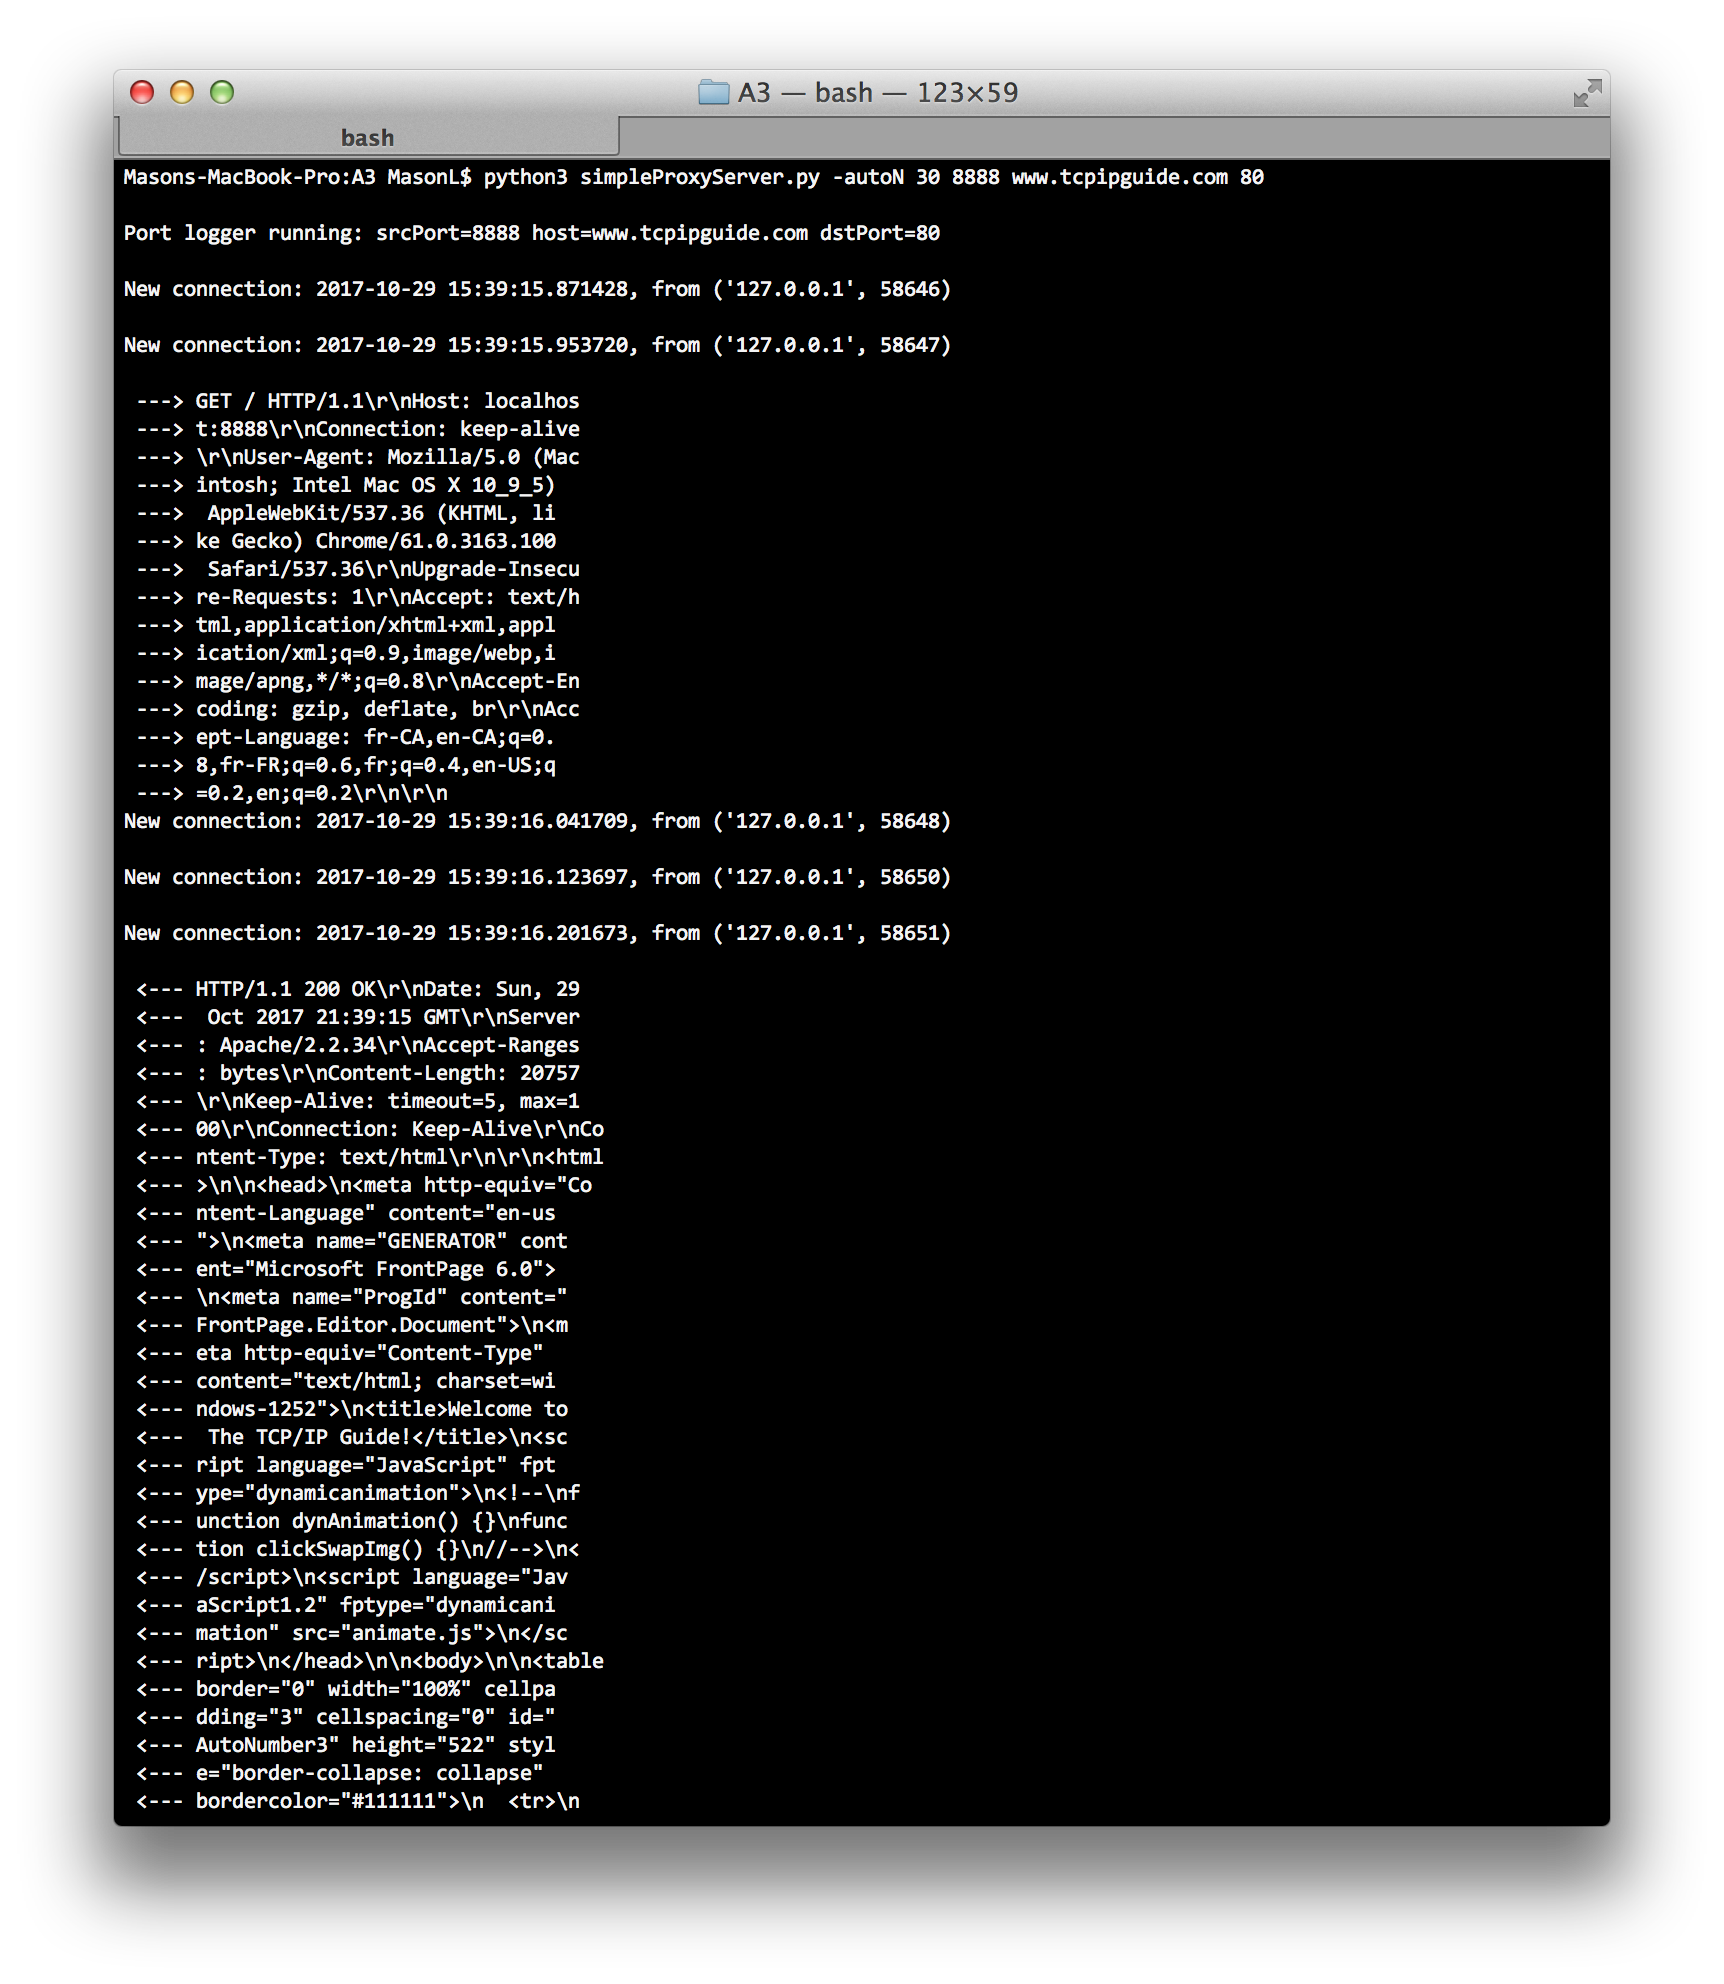
\includegraphics[scale=0.5, trim={0cm 0cm 0cm 0cm}, clip]{autoN_output}
	\caption{Initialization of proxy server with autoN formatting where n = 30}
	\end{figure}
	
	\subsection{Output - replace}
	\begin{figure}[H]
	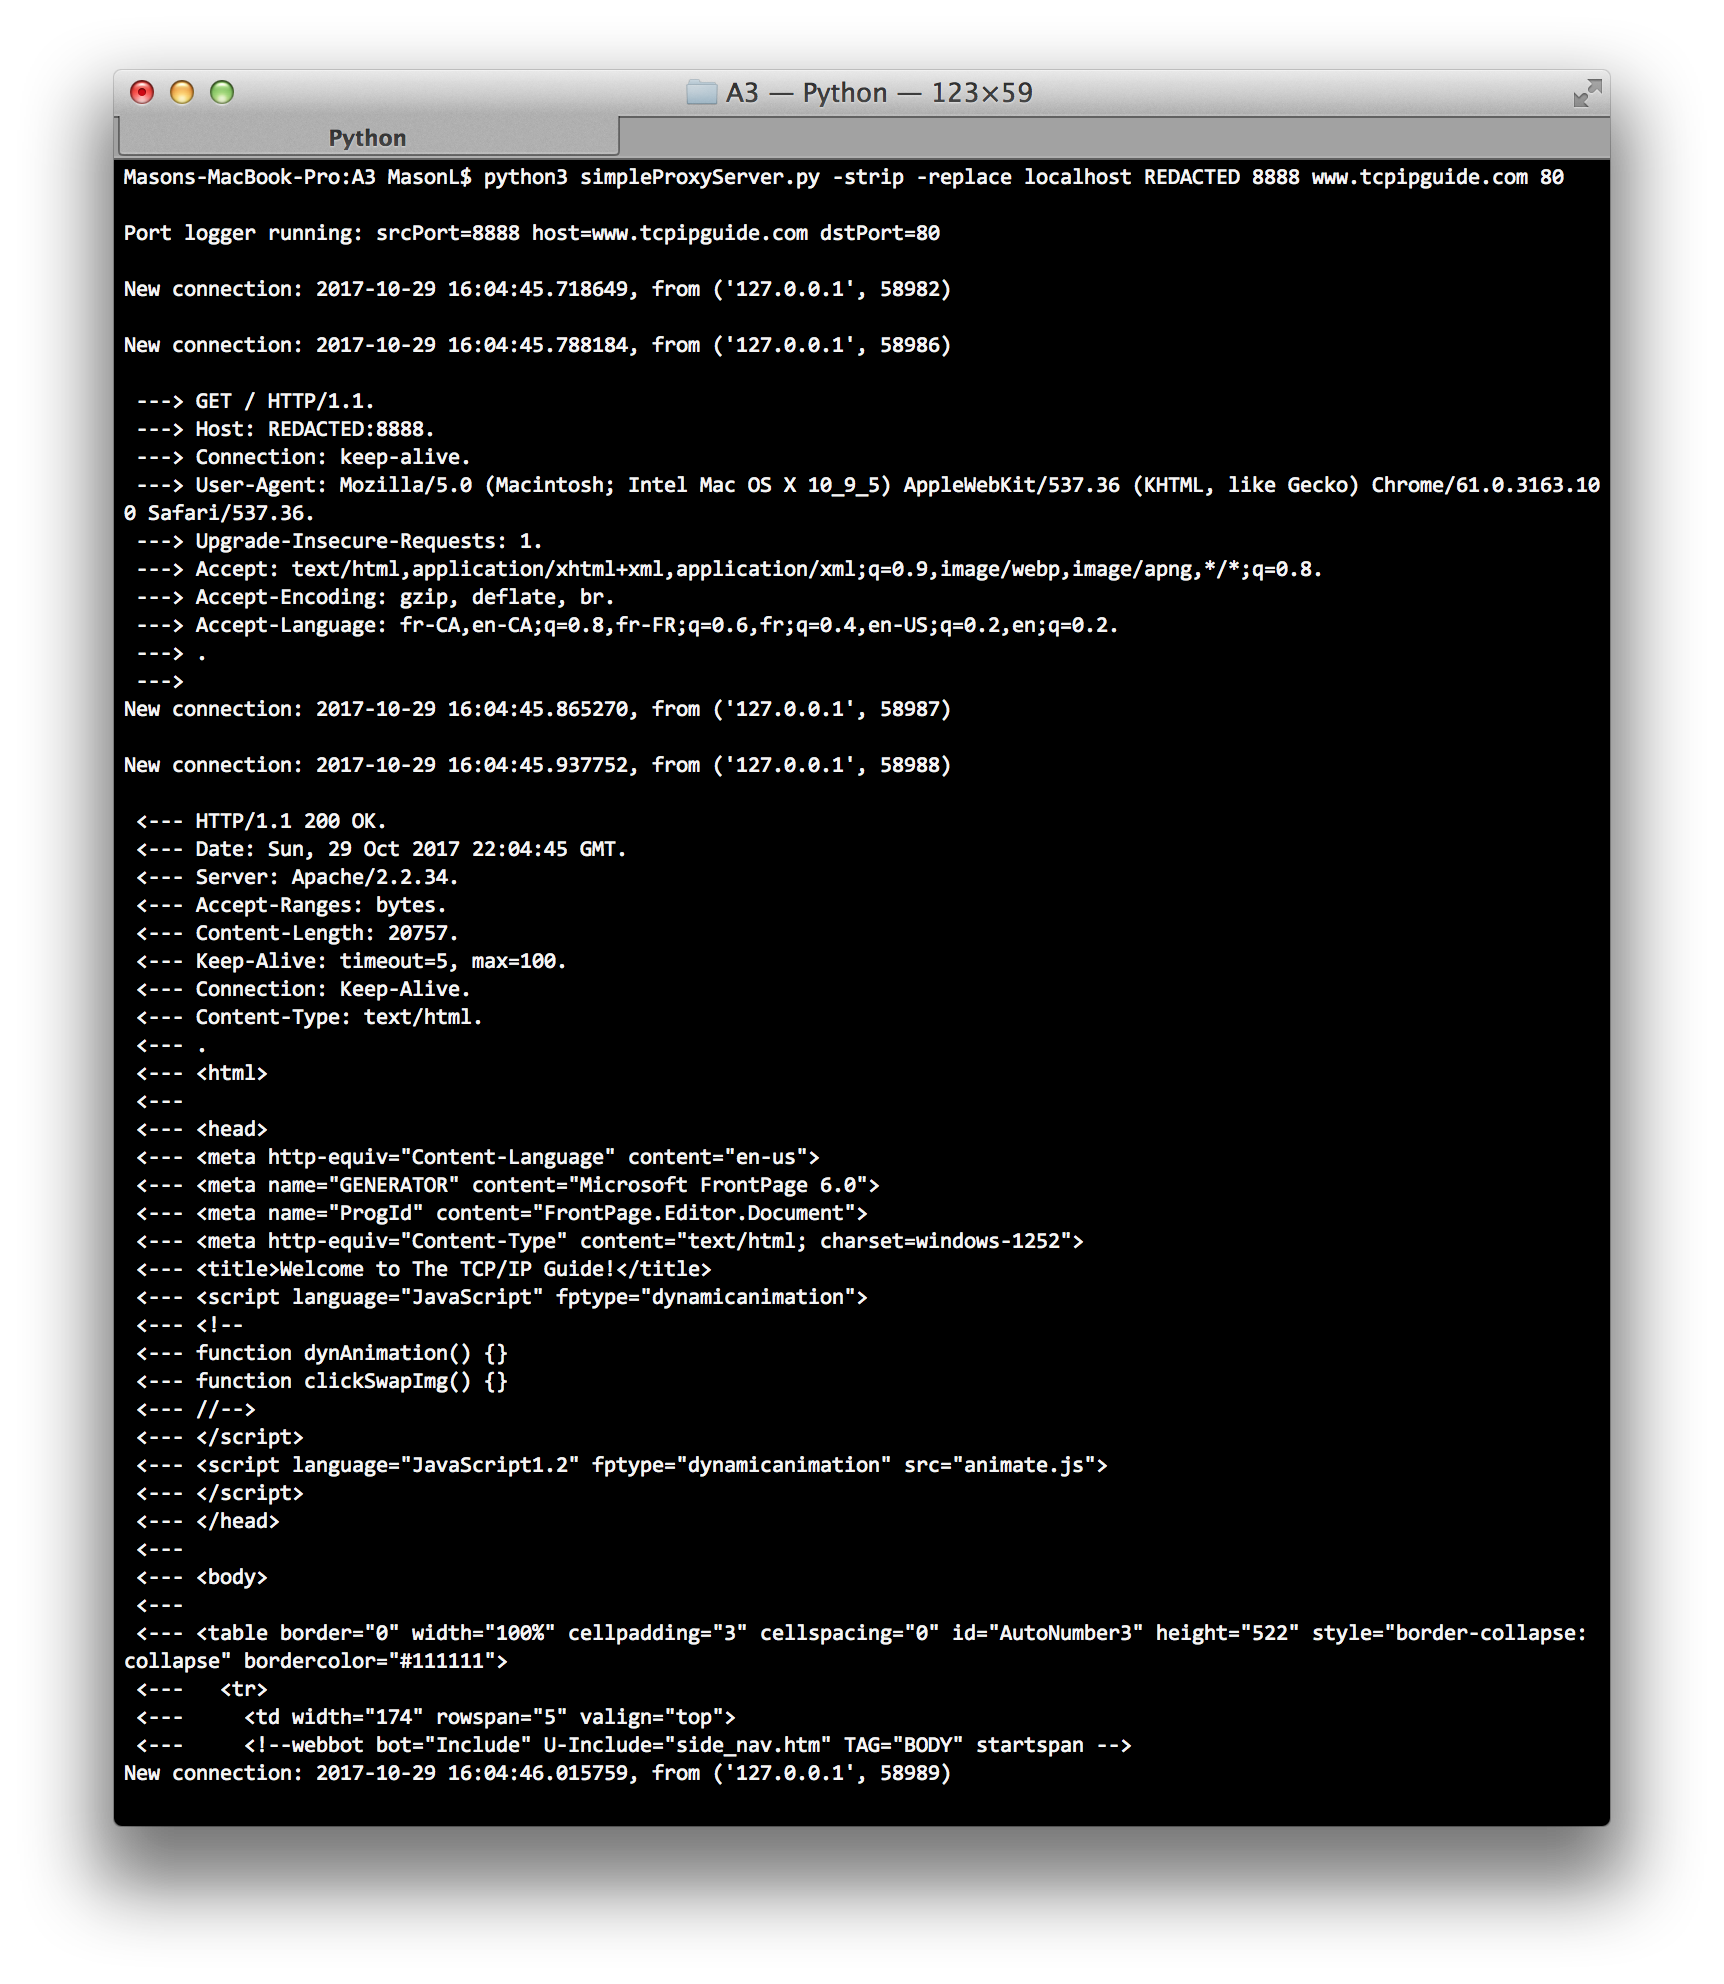
\includegraphics[scale=0.5, trim={0cm 0cm 0cm 0cm}, clip]{replace_output}
	\caption{Initialization of proxy server with replace formatting. All instances of `localhost' replaced with `REDACTED'}
	\end{figure}

\end{document}

